\documentclass{article}
\usepackage[utf8]{inputenc}

\title{Trabalho Prático 1 \\ Software Básico
\\ Ligador Simples}
\author{João Paulo Martino Bregunci - jpbregunci@gmail.com
\\ Ronald Davi Rodrigues Pereira - ronald.drp11@gmail.com}
\date{Novembro de 2016}

\usepackage{natbib}
\usepackage{graphicx}
\usepackage{indentfirst}

\begin{document}

\maketitle


\section{Introdução}
A tradução de cógido \textit{Assembly} para código de máquina é um dos problemas mais antigos da Ciência da Computação, dada a obvia dificuldade da programação diretamente em código de máquina. Desse problema, iniciou-se a proposta desse trabalho que será a construção de um \textit{Ligador} simples, o qual é capaz de gerar código executável para a máquina \textit{Wombat2}. Este dado \textit{Ligador} em questão criado irá possibilitar a execução de funções presentes em diversos outros arquivos, retornando posteriormente ao \textit{Program Counter} a próxima instrução depois que a função foi chamada.

O \textit{Ligador} ao final de todo o processo é capaz de gerar um único arquivo executável, o qual contém todas as funções existentes, sendo o endereço de chamada de todas esses funções recalculado para ajustar-se a chamada de qualquer outra função presente no arquivo executável final.


\begin{figure}[h!]
\centering
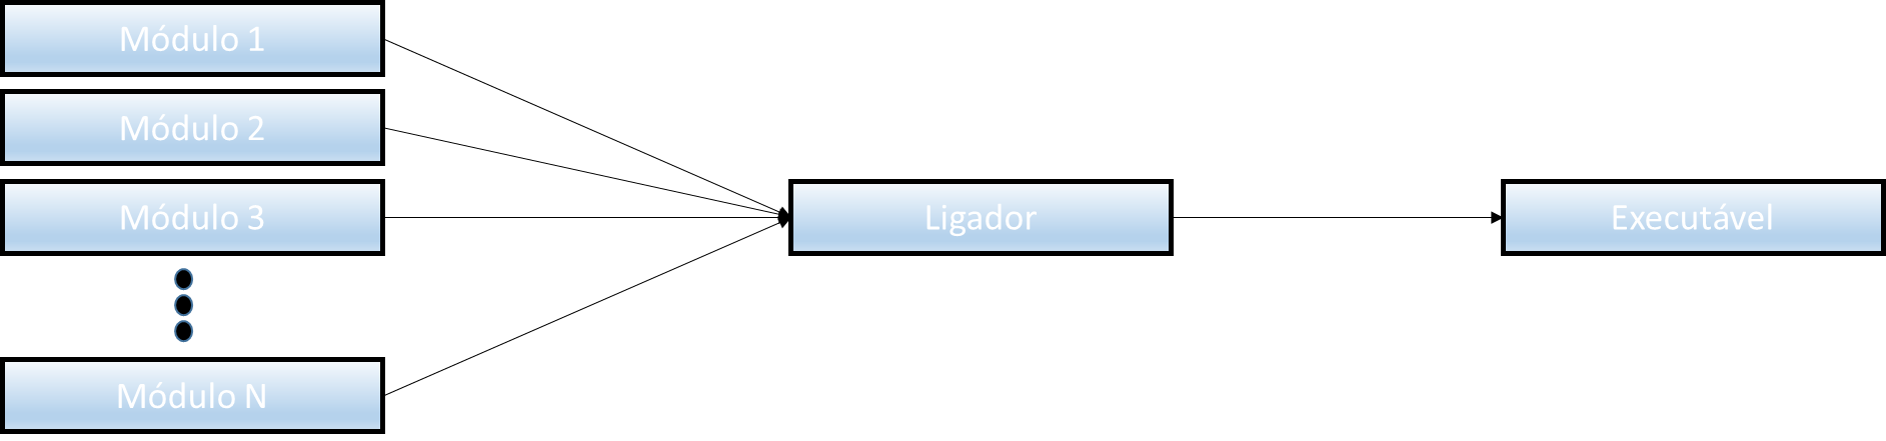
\includegraphics[scale=0.4]{ImagemTP2.png}
\caption{Diagrama que sintetiza o que o \textit{Ligador} faz}
\label{fig:trieExample}
\end{figure}

\section{Explanação do Problema}
\subsection{Apresentação do Problema}
Como enunciado anteriormente na Introdução, o problema consiste na implementação de \textit{Ligador} simples. Nesse contexto, notabiliza-se o maior problema o remanejamento do endereço das funções, ou seja, o recalculo do do endereço de memória no qual a função está depois que unem-se vários módulos ao executável principal.

\subsection{Solução Generalizada do Problema}
Para a construção do ligador deve-se pontuar, primariamente, algumas condições simples para que o programa seja capaz de gerar um executável final sem que exista qualquer tipo de comportamento inesperado. Tais condições enunciadas são:

\begin{enumerate}
  \item Não deve haver nenhum espaço (ou tabulação) antes de uma linha que contém somente comentários, ou seja, em linhas que contém exclusivamente comentários o primeiro carácter deve ser exclusivamente o ponto e vírgula.
  \item Não devem haver nenhuma linha escrita no fim do programa (após os .datas), mesmo que sejam comentários, a fim de evitar comportamentos irregulares durante a execução.
  \item Não devem haver nenhum rótulo (label) no meio do programa Assembly que não esteja declarado em outro local do código, a fim de evitar o evidente problema de referências para procedimentos inexistentes
  \item Labels devem começar com um \textit{underline}, tanto para jumps ou calls, a fim de padronizar de uma maneira simples a chamada de procedimentos
\end{enumerate}


\subsection{Implementação das Passagens}
Na primeira passagem há a criação de duas listas encadeadas, as quais são as duas tabelas de símbolos. Uma dessas tabelas contem todos os \textit{.data}, que serão prontamente substituidos e a outra tabela contem referências para os PC (\textit{program counter}) de labels encontradas na primeira passagem do \textit{Assembler}. Escolheram-se listas encadeadas para a estruturação da Tabela de Símbolos, pois não existem problemas eventuais na procura de elementos da lista em \textit{O(n)}, já que o número de \textit{labels} e \textit{.data} não prejudica severamente a performance do código.
Depois disso se realiza o processo corriqueiro de decodificação por meio de uma série de \textit{if, else if e else} para a leitura da instrução e a tradução do valores de eventuais registradores para os respectivos valores binários. Após todo esse processo se encontra o arquivo executável gerado.

\section{Casos de Teste}

\section{Conclusão}

Por meio desse trabalho foi possível expandir ainda mais o conhecimento sobre a geração de código máquina, a partir de um código \textit{Assembly}. Foi gerado ao final desse trabalho, um \textit{Ligador} completamente funcional capaz de gerar eficientemente um código executável para a máquina \textit{Wombat2}, utilizando para isso, diversos procedimentos de vários módulos simultaneamente.


\begin{thebibliography}{9}

\bibitem{knuthwebsite} 
Colby College, Official CPUsim Website
\\\texttt{http://www.cs.colby.edu/djskrien/CPUSim/}
\end{thebibliography}
\end{document}

